%────────────────────── Capítulo 4 — Resultados ────────────────────────
% Análisis de los resultados, a ser posible sobre máquinas reales.
% Solo datos medidos o simulados por nosotros; las simulaciones se
% etiquetan como tales. Las figuras salen de los scripts de análisis.
\chapter{Resultados}
\label{cap:resultados}

\section{Validación del análisis con trazas simuladas}
\label{sec:validacion-simulada}
% Todos los números y figuras de esta sección salen de:
%   uv run python -m analisis.run_all
% (analisis/experiments.py, analisis/figures.py y analisis/config.py).
% Los resultados numéricos quedan en analisis/salida/resultados.json, que no
% se sube al repositorio porque se regenera con la misma semilla.

Antes de medir nada conviene comprobar que el ataque está bien implementado y
saber qué cabe esperar de él. Para eso se generan \emph{trazas sintéticas} con
el modelo de fuga de la \cref{sec:cpa} ---peso de Hamming del valor intermedio
más ruido gaussiano--- y se atacan con el mismo código que después se aplicará
a las trazas medidas. \textbf{Todo lo que aparece en esta sección es
simulación}: no son medidas de ningún montaje y no dicen nada sobre el
microcontrolador, que todavía no se ha instrumentado.

\subsection{Modelo de las trazas simuladas}

Cada traza sintética se construye sumando a la fuga buscada cuatro
perturbaciones que también aparecen en una medida real:

\begin{equation}
  T_i[t] = \underbrace{b_i}_{\text{offset}}
         + \underbrace{d_i[t]}_{\text{deriva}}
         + \underbrace{n_i[t]}_{\text{ruido}}
         + \sum_{r} g_r \cdot \operatorname{HW}\!\left(V_i^{(r)}\right) \cdot k[t - t_r],
  \label{eq:modelo-traza}
\end{equation}

donde $V^{(1)}_i = \mathrm{SBox}(p_i \oplus k)$ es la salida de la S-box de la
primera ronda, $V^{(10)}_i = \mathrm{InvSBox}(c_i \oplus k)$ la entrada de la
S-box de la última, $k[\cdot]$ un núcleo $(0{,}5,\,1{,}0,\,0{,}5)$ que reparte
cada operación en tres muestras consecutivas y $t_r$ el instante central de la
operación del byte $r$. La separación entre ventanas es de dos muestras, como
correspondería a un recorrido byte a byte del estado en el microcontrolador.
La relación señal-ruido se define sobre la potencia de la fuga,
$\mathrm{SNR} = \operatorname{Var}\!\left(\sum_r g_r \operatorname{HW}(V^{(r)})\right) / \sigma_n^2$,
que es lo que permite comparar campañas con distinto ruido. El desplazamiento
$b_i$ es constante dentro de una traza: infla la varianza de la traza y por
tanto rebaja algo la correlación medida, pero no cambia el orden de los
candidatos, porque la correlación de Pearson lo elimina.

Los parámetros concretos de la campaña de referencia ---4000 trazas de 96
muestras, $\mathrm{SNR} = 0{,}1$, semilla \num{20261018}--- están en
\texttt{analisis/config.py} y se guardan en el JSON de resultados, de modo que
la ejecución se puede repetir exactamente. La \cref{fig:sim-trazas} muestra
cómo son.

\begin{figure}[htbp]
  \centering
  % Generada por analisis/figures.py::figure_synthetic_traces
  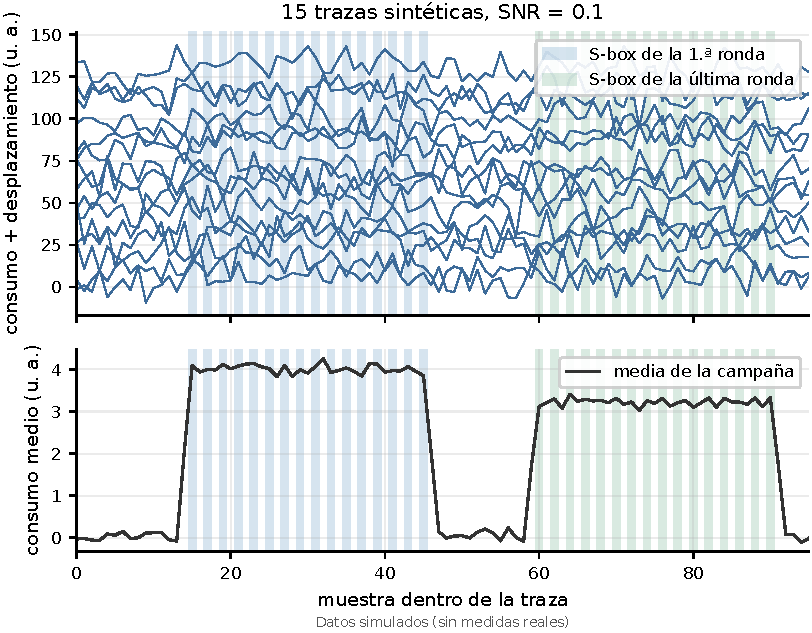
\includegraphics[width=\textwidth]{sim-trazas.pdf}
  \caption{Trazas sintéticas de la campaña de referencia (arriba, quince
    trazas superpuestas con un desplazamiento vertical para distinguirlas) y
    su media (abajo). Las bandas señalan la ventana temporal de la S-box de la
    primera ronda (azul) y de la última (verde). En la media se ve el escalón
    del peso de Hamming de cada byte del estado. \textbf{Datos simulados.}}
  \label{fig:sim-trazas}
\end{figure}

\subsection{Comprobación del AES}

El valor intermedio que ataca el CPA tiene que ser exactamente el de la norma,
o el ataque buscaría una clave distinta de la real. La implementación de
referencia se comprueba contra los vectores de ejemplo del FIPS-197
\cite{nist2023fips197}: el ejemplo del apéndice~B, el caso trivial del apéndice
C.1 y dos casos con clave o texto claro todo a uno. En los cuatro se verifica
el cifrado y el descifrado, y además se comprueba que la versión vectorizada
---la que genera las trazas--- produce byte a byte el mismo resultado que la
versión directa. Estas comprobaciones forman parte de
\texttt{uv run python -m analisis.tests} y se ejecutan antes de generar
cualquier figura.

\subsection{Recuperación de la clave}

La \cref{fig:sim-cpa-correlacion} muestra el resultado central del ataque sobre
la campaña de referencia. Arriba está el coeficiente de correlación del
candidato correcto de cada uno de los 16 bytes; abajo, el mayor de los 255
candidatos falsos. La diferencia es nítida: el candidato correcto llega a
$|\rho| \approx \num{0,22}$ justo en la ventana de su byte, mientras que
ningún candidato falso pasa de $\num{0,07}$. Los 16 bytes de la clave se
recuperan con 4000 trazas, tanto atacando la primera ronda
($\overline{|\rho|} = \num{0,221}$, mínimo $\num{0,212}$) como la última
($\overline{|\rho|} = \num{0,184}$). La cota teórica para esta campaña es
$\rho_{\max} = \sqrt{\mathrm{SNR}/(1+\mathrm{SNR})} = \num{0,302}$; la
diferencia se explica por el desplazamiento por traza de la
\cref{eq:modelo-traza}, que engorda la varianza de la traza y baja la cota a
$\num{0,286}$ en estas condiciones.

\begin{figure}[htbp]
  \centering
  % Generada por analisis/figures.py::figure_correlation_over_time
  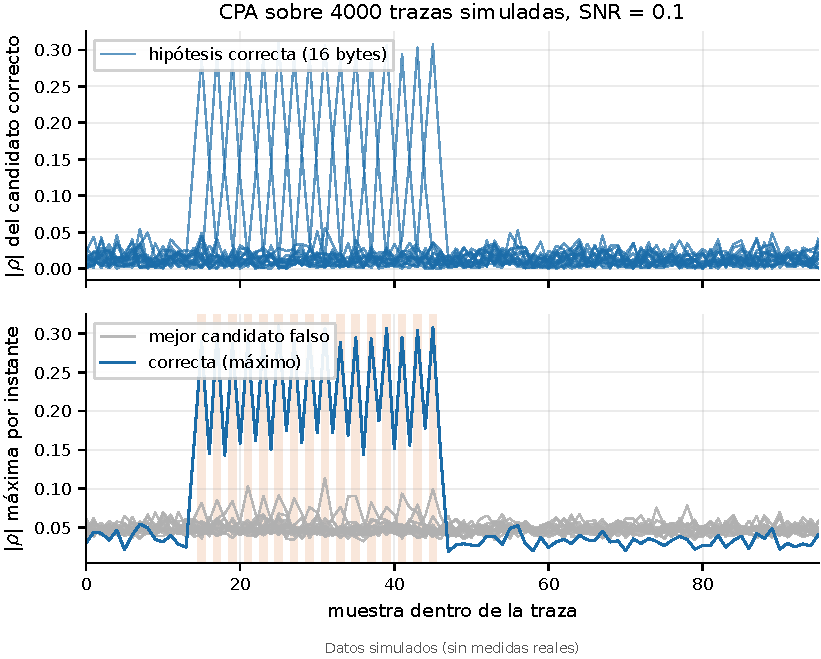
\includegraphics[width=\textwidth]{sim-cpa-correlacion.pdf}
  \caption{Correlación de Pearson frente al tiempo, sobre 4000 trazas
    simuladas con $\mathrm{SNR} = 0{,}1$. Arriba, el candidato correcto de
    cada uno de los 16 bytes; abajo, el mejor candidato falso de cada byte,
    que se queda muy por debajo. Las bandas marcan las ventanas de la S-box.
    \textbf{Datos simulados.}}
  \label{fig:sim-cpa-correlacion}
\end{figure}

La \cref{fig:sim-candidatos} ordena los 256 candidatos por su pico de
correlación y muestra en qué puesto queda el correcto. La separación entre el
primero y el resto es el margen del ataque: $\overline{\Delta|\rho|} =
\num{0,146}$ en la primera ronda, y el candidato correcto es el primero en los
16 bytes. El ataque acierta también en el \emph{tiempo}: el pico del byte $j$
cae en la muestra $15 + 2j$, que es donde el simulador colocó su operación.

\begin{figure}[htbp]
  \centering
  % Generada por analisis/figures.py::figure_peaks_per_candidate
  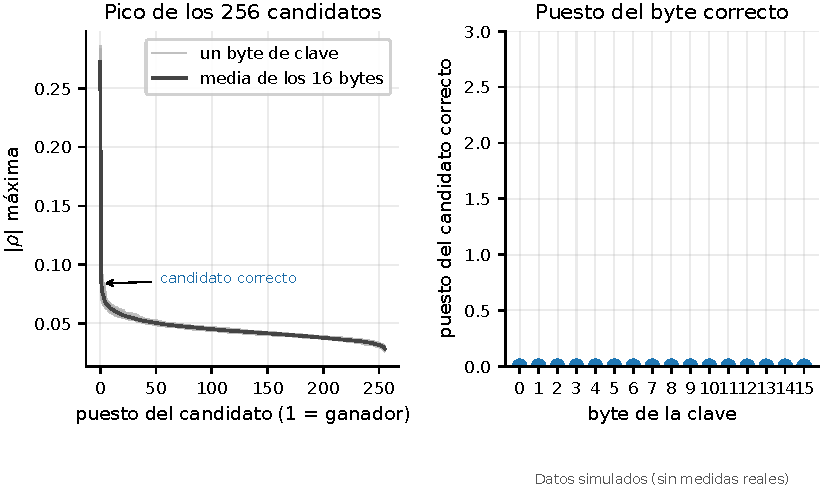
\includegraphics[width=\textwidth]{sim-candidatos.pdf}
  \caption{Izquierda: pico de $|\rho|$ de los 256 candidatos de cada byte,
    ordenados de mayor a menor, más la media de los 16 bytes. Derecha: puesto
    que ocupa la hipótesis correcta en cada byte (1 = ganador).
    \textbf{Datos simulados.}}
  \label{fig:sim-candidatos}
\end{figure}

\subsection{Cuántas trazas y cuánto ruido}

El número de trazas y el ruido son los dos factores que deciden si el ataque
funciona. Para medirlo se repite el CPA completo sobre 60 campañas
independientes de 3000 trazas ---con clave y textos claros nuevos en cada
una--- en nueve niveles de ruido, y se anota en qué puesto queda el byte
correcto de cada posición. El resultado está en la
\cref{fig:sim-rango} para la campaña de referencia y en la
\cref{tab:sim-ruido} para todos los niveles.

\begin{figure}[htbp]
  \centering
  % Generada por analisis/figures.py::figure_rank_curve y figure_noise_scaling
  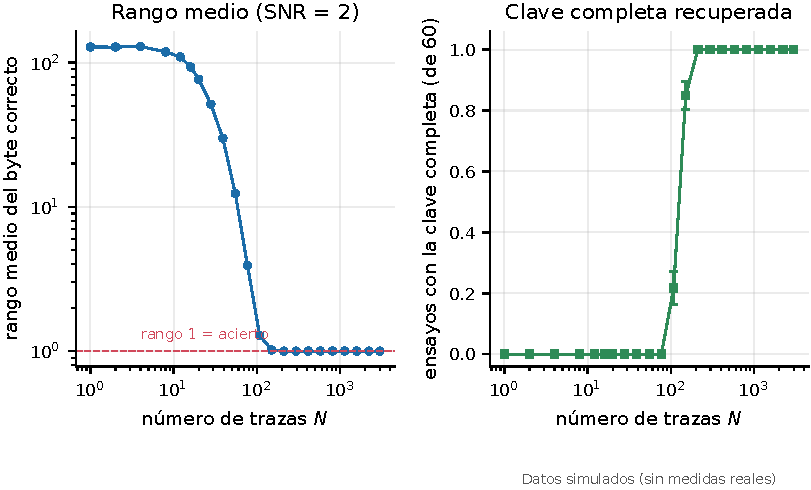
\includegraphics[width=\textwidth]{sim-rango.pdf}
  \caption{Izquierda: rango medio del byte correcto frente al número de trazas
    ($\mathrm{SNR} = 0{,}1$, media de 60 ensayos). Derecha: proporción de
    ensayos en los que se recuperan los 256 bits. \textbf{Datos simulados.}}
  \label{fig:sim-rango}
\end{figure}

\begin{table}[htbp]
  \centering
  \caption{Trazas necesarias para recuperar los 256 bits en función del ruido.
    «N para el 90~\%» es el primer número de trazas en el que la media de los
    60 ensayos lo consigue; «N mediana», la mediana del primer instante en que
    lo consigue cada ensayo. La última columna es el pico medio de $|\rho|$ del
    candidato correcto con 3000 trazas. \textbf{Datos simulados.}}
  \label{tab:sim-ruido}
  \begin{tabular}{S[table-format=1.3] S[table-format=4.0] S[table-format=4.0] S[table-format=1.3]}
    \toprule
    {SNR} & {N para el 90~\%} & {N mediana} & {pico de $|\rho|$} \\
    \midrule
    2      & 211  & 151  & 0,515 \\
    1      & 211  & 211  & 0,466 \\
    0,5    & 295  & 295  & 0,400 \\
    0,2    & 578  & 413  & 0,300 \\
    0,1    & 1133 & 809  & 0,227 \\
    0,05   & 1586 & 1586 & 0,166 \\
    0,02   & \multicolumn{1}{c}{$>$3000} & \multicolumn{1}{c}{$>$3000} & 0,108 \\
    0,01   & \multicolumn{1}{c}{$>$3000} & \multicolumn{1}{c}{$>$3000} & 0,079 \\
    0,005  & \multicolumn{1}{c}{$>$3000} & \multicolumn{1}{c}{$>$3000} & 0,062 \\
    \bottomrule
  \end{tabular}
\end{table}

\begin{figure}[htbp]
  \centering
  % Generada por analisis/figures.py::figure_noise_scaling
  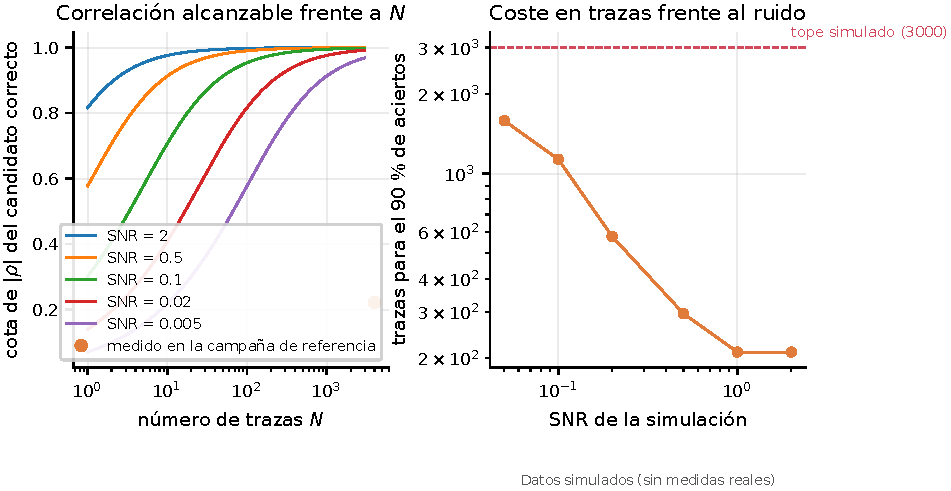
\includegraphics[width=\textwidth]{sim-ruido.pdf}
  \caption{Izquierda: cota teórica de $|\rho|$ en función del número de trazas
    para varios niveles de ruido, con el valor medido en la campaña de
    referencia. Derecha: trazas necesarias para recuperar los 256 bits en el
    90~\% de los ensayos. \textbf{Datos simulados.}}
  \label{fig:sim-ruido}
\end{figure}

Los resultados siguen la ley esperada: la correlación crece como
$\sqrt{N\,\mathrm{SNR}/(1 + N\,\mathrm{SNR})}$, de modo que hacer el ataque
viable con diez veces menos trazas exige diez veces menos ruido. Por debajo de
$\mathrm{SNR} = 0{,}02$ la campaña de 3000 trazas ya no basta y el candidato
correcto se queda fuera del primer puesto en más de la mitad de los ensayos.
Hay que insistir en que estos números son propiedad del \emph{modelo}, no del
montaje: fijan el orden de magnitud que habrá que comparar con las medidas
reales, y solo entonces se podrá decir si el montaje se parece a la simulación.

\subsection{Comparación con el DPA}

El DPA clásico separa las trazas según un único bit del valor intermedio
\cite{kocher1999dpa}, así que aprovecha mucha menos información que el modelo
de peso de Hamming del CPA \cite{brier2004cpa}. La \cref{fig:sim-dpa-cpa} lo
cuantifica sobre la misma campaña de 2000 trazas con $\mathrm{SNR} = 0{,}1$: el
CPA recupera los 16 bytes, mientras que el mejor de los ocho bits del DPA
recupera 8 y el peor, uno solo. La comparación justifica atacar con el peso de
Hamming completo (o con un modelo de fuga más rico) en cuanto el ruido aprieta.

\begin{figure}[htbp]
  \centering
  % Generada por analisis/figures.py::figure_dpa_vs_cpa
  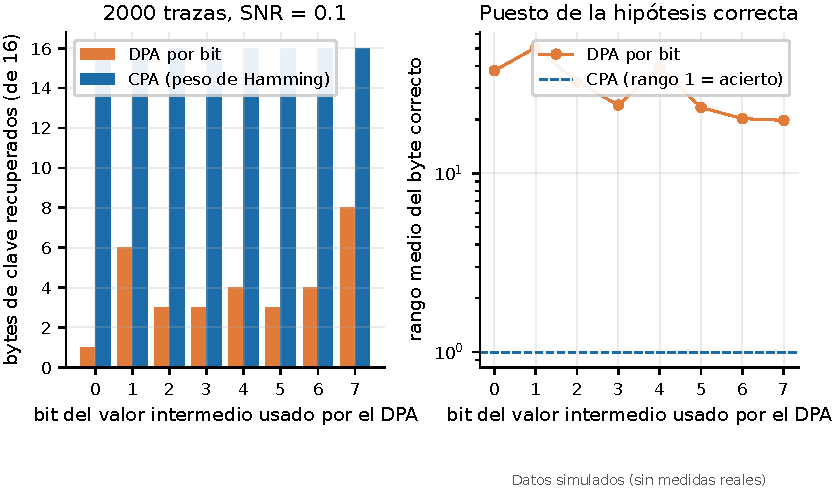
\includegraphics[width=\textwidth]{sim-dpa-cpa.pdf}
  \caption{Izquierda: bytes de clave recuperados por el DPA de cada bit y por
    el CPA sobre la misma campaña de 2000 trazas simuladas
    ($\mathrm{SNR} = 0{,}1$). Derecha: puesto medio de la hipótesis correcta.
    \textbf{Datos simulados.}}
  \label{fig:sim-dpa-cpa}
\end{figure}

\section{Calidad de la captura}
% TODO: traza real, alineación con el trigger, ruido, frecuencia de
% muestreo efectiva frente al reloj del microcontrolador.

\section{Recuperación de la clave}
% TODO: correlación frente al tiempo, correlación máxima por candidato,
% rango de la clave correcta frente al número de trazas y comparación de
% la clave recuperada con la de laboratorio. (Con trazas reales, fase 5.)

\section{Limitaciones}
% TODO: qué condiciones del montaje favorecen o dificultan el ataque.
